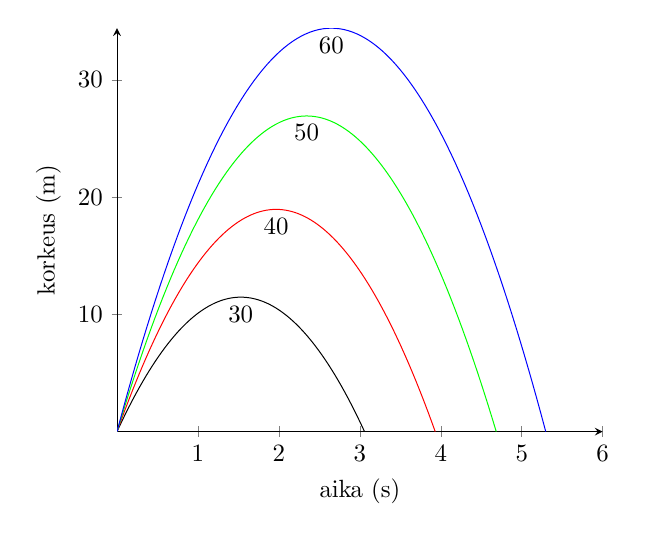
\begin{tikzpicture}[scale=0.9]
\begin{axis}[axis lines=center,
            xlabel={aika (s)},
            xlabel near ticks,
            ylabel={korkeus (m)},
            ylabel near ticks,
            xmin=0, xmax=6, ymin=0]
\addplot[color=black,
        domain=0:30*sin(30)/(0.5*9.81),
        samples=101]
        {30*sin(30)*x - 0.5*9.81*x^2}
        node[color=black, midway, below]{\ang{30}};
\addplot[color=red,
        domain=0:30*sin(40)/(0.5*9.81),
        samples=101]
        {30*sin(40)*x - 0.5*9.81*x^2}
        node[color=black, midway, below]{\ang{40}};
\addplot[color=green,
        domain=0:30*sin(50)/(0.5*9.81),
        samples=101]
        {30*sin(50)*x - 0.5*9.81*x^2}
        node[color=black, midway, below]{\ang{50}};
\addplot[color=blue,
        domain=0:30*sin(60)/(0.5*9.81),
        samples=101]
        {30*sin(60)*x - 0.5*9.81*x^2}
        node[color=black, midway, below]{\ang{60}};
\end{axis}
\end{tikzpicture}